\section{Experiments}\label{sec:experiment}
We experimentally evaluated the performance and quality of our methodology \cref{subsec:heuristics},
and compared it against the exhaustive approach in Section~\ref{TOADD}. In the following,
\cref{subsec:experiments_infrastructure} presents the simulator and testing infrastructure adopted in our experiments, as well as the complete experimental settings; \cref{subsec:experiments_performance} analyses the performance of our solution in terms of execution time; \cref{subsec:experiments_quality} presents the quality of our heuristic algorithm in terms of the metrics in \cref{subsec:metrics}.

\subsection{Testing Infrastructure and Experimental Settings}\label{subsec:experiments_infrastructure}
Our testing infrastructure is a Swift-based simulator of a service-based ecosystem, including service execution, comparison, and composition. The simulator first defines the pipeline template as a sequence of nodes in the range \hl{x-y}. We recall that alternative nodes are modeled in different pipeline templates, while parallel nodes only add a fixed execution time that is negligible and do not affect the quality of our approach. Each node is associated with a (set of) policy with transformations varying in three classes: \hl{a,b,c}. A set of functionally-equivalent candidate services is randomly generated, each service having a profile...\hl{to conclude}. 
Upon setting up the pipeline template, the sliding window size is configured and our methodology for pipeline instance generation starts. %The simulator selects a subset of nodes along with their corresponding candidate services.
The simulator calculates all possible pipeline instances, that is, it instantiates all nodes with a service according to the selected window size. For each node, the simulator calculates a quality metric, selecting the first service from the optimal combination in the sliding window, then shifting the window by step 1.
When the end of the node list is reached, or when the window size equals the node count, the simulator computes the optimal service combination for the remaining nodes and the pipeline instance is generated.
\hl{NON MI E' CHIARISSIMA To ensure that each service is interdependent within a combination, a hash function is employed. This function generates weights that services use to simulate transformations (data removal) mandated by the specified policies.}
The simulator is used to assess the performance and quality of our sliding window heuristic in Section \ref{sec:heuristics} for the generation of the best pipeline instance (Section \ref{sec:instance}).
% Performance measures the heuristics execution time in different settings, while quality compares the results provided by our heuristics in terms of selected services with the optimal solution retrieved using the exhaustive approach.
%We note that the exhaustive approach generates the best pipeline instance by executing all possible combinations of candidate services.
%The emulator simplifies the execution of the service composition by removing the service selection phase, which is not relevant for the purpose of the experiment.
Our experiments have been run on a workstation equipped with a 2.40GHz i5-8279U CPU with 16GB RAM and a 512GB SSD.
Each experiment was repeated ten times and the results averaged to improve the reliability of the data.

\usetikzlibrary{positioning}
\usetikzlibrary{backgrounds}

\begin{figure}[!t]
  \centering
  \newcommand{\function}{$\instanceChartAnnotation{}$}
  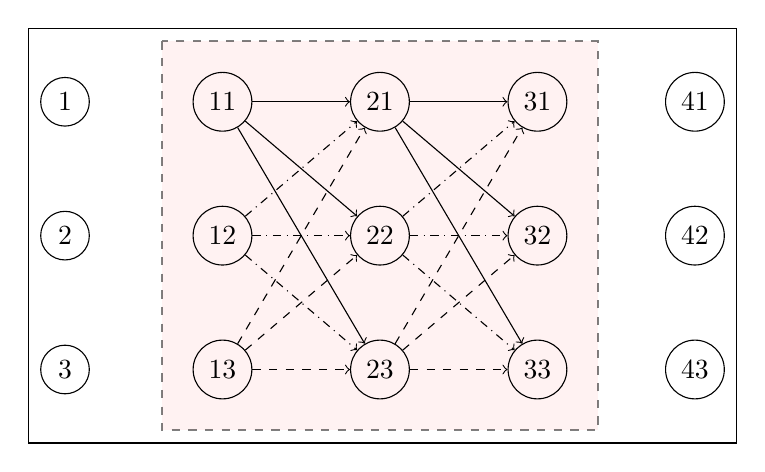
\begin{tikzpicture}[framed]
    \node[draw, circle] (s41) at (1,1.7) {$\sii{1}$};
    \node[draw, circle] (s42) at (1,0) {$\sii{2}$};
    \node[draw, circle] (s43) at (1,-1.7) {$\sii{3}$};

    \node[draw, circle] (s1) at (3,1.7) {$\sii{11}$};
    \node[draw, circle] (s2) at (3,0) {$\sii{12}$};
    \node[draw, circle] (s3) at (3,-1.7) {$\sii{13}$};

    \node[draw, circle] (s11) at (5,1.7) {$\sii{21}$};
    \node[draw, circle] (s12) at (5,0) {$\sii{22}$};
    \node[draw, circle] (s13) at (5,-1.7) {$\sii{23}$};

    \node[draw, circle] (s21) at (7,1.7) {$\sii{31}$};
    \node[draw, circle] (s22) at (7,0) {$\sii{32}$};
    \node[draw, circle] (s23) at (7,-1.7) {$\sii{33}$};

    \node[draw, circle] (s31) at (9,1.7) {$\sii{41}$};
    \node[draw, circle] (s32) at (9,0) {$\sii{42}$};
    \node[draw, circle] (s33) at (9,-1.7) {$\sii{43}$};


    % \draw[->] (node2) -- (node3);
    \draw[->] (s1) -- (s11);
    \draw[->] (s1) -- (s12);
    \draw[->] (s1) -- (s13);

    \draw[->,dashdotted] (s2) -- (s11);
    \draw[->,dashdotted] (s2) -- (s12);
    \draw[->,dashdotted] (s2) -- (s13);

    \draw[->,dashed] (s3) -- (s11);
    \draw[->,dashed] (s3) -- (s12);
    \draw[->,dashed] (s3) -- (s13);


    \draw[->] (s11) -- (s21);
    \draw[->] (s11) -- (s22);
    \draw[->] (s11) -- (s23);

    \draw[->,dashdotted] (s12) -- (s21);
    \draw[->,dashdotted] (s12) -- (s22);
    \draw[->,dashdotted] (s12) -- (s23);

    \draw[->,dashed] (s13) -- (s21);
    \draw[->,dashed] (s13) -- (s22);
    \draw[->,dashed] (s13) -- (s23);


    \begin{scope}[on background layer]
      \draw[thick, dashed, fill=red!10, opacity=0.5]
      ([shift={(-0.5,0.5)}]s1.north west) rectangle ([shift={(0.5,-0.5)}]s23.south east);

    \end{scope}
  \end{tikzpicture}
  \caption{Service composition instance}
  \label{fig:service_composition_instance}
\end{figure}

\subsection{Perfomance}\label{subsec:experiments_performance}
% \subsection{performance}
% \begin{itemize}
%   \item Finestra scorrevole da 1 a N=Nodi
%   \item Servizi 5 a 20 passo 5 + 50??
%   \item
% \end{itemize}
% \subsection{Metriche/Euristiche}
We first calculated the execution time required by our exhaustive solution.
We incrementally varied the number of nodes and the number of services per node.
The results of these evaluations are presented in \cref{fig:perf_exhaustive}.
As anticipated, the trend in execution times is exponential. \cref{fig:perf_exhaustive} displays the execution time plots,
clearly showing that as the number of nodes increases, the execution time grows exponentially.
Execution times for up to 5 nodes and 6 services were computed directly,
while the remaining data points were obtained through interpolation.
Subsequently, the logical extension of this empirical inquiry involves evaluating the execution time efficiency attributable to the implementation of the sliding window heuristic.

We then evaluated our heuristics to quantify the execution time reduction achieved through the application of heuristics.
In this context, the number of nodes and services per node was incrementally increased,
with the addition of a sliding window whose size was progressively enlarged in each experiment.
The outcomes are depicted in \cref{fig:perf_window}, and as expected,
we observed a marked reduction in execution times with the implementation of the sliding window heuristic.
This empirical evidence highlights the heuristic's ability to reduce computational demands,
an aspect that becomes increasingly pivotal as the problem's complexity grows.
The use of a logarithmic scale to illustrate the results linearizes the exponential growth associated with the exhaustive method,
offering a clear visual confirmation of the heuristic's efficiency in decreasing computational time.


\subsection{Quality}\label{subsec:experiments_quality}
We finally evaluated the quality of our heuristic comparing, where possible, its results with the optimal solution retrieved by executing the exhaustive approach. The latter executes with window size equals to the number of nodes and provides the best, among all possible, solution.

We recall that we considered three different setting, confident, diffident, average, varying the policy transformations, that is, the amount of data removal at each node. Setting confident assigns to each policy a transformation that changes the amount of data removal in the interval [x,y] (Jaccard coefficient) or decreases the probability distribution dissimilarity in the interval [x,y] (Jensen-Shannon Divergence). Setting diffident assigns to each policy a transformation that changes the amount of data removal in the interval [x,y] (Jaccard coefficient) or decreases the probability distribution dissimilarity in  the interval [x,y] (Jensen-Shannon Divergence). Setting average assigns to each policy a transformation that changes the amount of data removal in the interval [x,y] (Jaccard coefficient) or decreases the probability distribution dissimilarity in  the interval [x,y] (Jensen-Shannon Divergence).

% \hl{DOBBIAMO SPIEGARE COSA ABBIAMO VARIATO NEGLI ESPERIMENTI E COME, WINDOW SIZE, NODI, ETC.

%   LE IMMAGINI CHE ABBIAMO SONO SOLO QUELLE 5? POSSIAMO ANCHE INVERTIRE GLI ASSI E AGGIUNGERE VISUALI DIVERSE}

\cref{fig:quality_window} presents our results with setting \hl{confident} and metric Jaccard coefficient. \cref{fig:quality_window}(a)--(e) \hl{aggiungere le lettere e uniformare l'asse y} present the retrieved quality varying the number of nodes in [3, 7], respectively. Each figure in \cref{fig:quality_window}(a)--(e) varies the number of candidate services at each node in the range [2, 6] and the window size W in the range [1, $|$nodes$|$].
\hl{aggiungiamo i numeri piu significativi (asse y).} 
From the results, some clear trends emerge. As the number of nodes increases, the metric values tend to decrease (better data quality) as the window size increases across different node configurations.
This suggests that the heuristic performs better when it has a broader perspective of the data and services. The trend is consistent across all node cardinalities (from three to seven), indicating that the heuristic's enhanced performance with larger window sizes is not confined to a specific setup but rather a general characteristic of its behavior.
Finally, the data suggest that while larger window sizes generally lead to better performance,
there might exist a point where the balance between window size and performance is optimized. \hl{For instance, ...}
Beyond this point, the incremental gains in metric values may not justify the additional computational resources or the complexity introduced by larger windows.

\hl{RIPETERE PER TUTTI I SETTINGS}


\begin{figure}
  \includegraphics[width=0.95\columnwidth]{graphs/exhaustive_performance.eps}
  \caption{Exhaustive execution time evaluation. The x-axis represents the number of services, while the y-axis represents the execution time in seconds. The execution time is expressed both in linear and logarithmic scales.}
  \label{fig:perf_exhaustive}
\end{figure}

\begin{figure}[!t]
  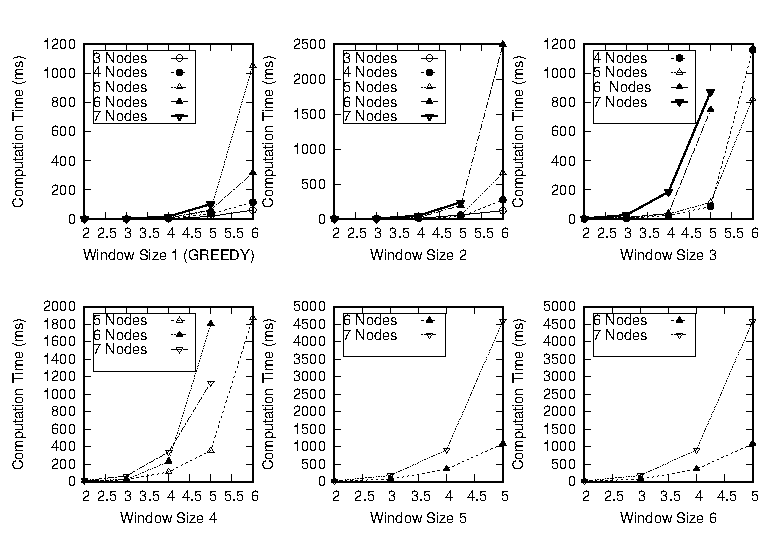
\includegraphics[width=0.95\columnwidth]{graphs/window_performance.eps}
  \caption{Preliminary performance evaluation.\hl{METTERE LE 4 IMG NON UN'UNICA EPS}}
  \label{fig:perf_window}
\end{figure}


\begin{figure}[!t]
  \includegraphics[width=0.95\columnwidth]{graphs/window_quality.eps}
  \caption{Quality evaluation.\hl{METTERE LE 4 IMG NON UN'UNICA EPS}}
  \label{fig:quality_window}
\end{figure}
